\chapter{Results}
This chapter presents the main numerical results of the thesis. The first part analyzes the optimized PMM chains obtained from the basin-hopping optimization procedure. The optimized parameters are compared across system sizes and interaction strengths, and the resulting Hamiltonians are evaluated using the spectral and local Majorana diagnostics introduced in the previous chapters.

The second part focuses on braiding. Based on the post-optimization diagnostics, the most promising optimized configuration is selected as the building block for a three-subsystem braiding geometry. The braid analysis begins with a controlled ground-state benchmark, comparing the energy-level Majorana reference model, the projected microscopic junction model, and the projected local-operator model. The projected microscopic junction is used to identify which low-energy Majorana channel is selected by physical endpoint couplings. The selected projected local Majorana operators, denoted by $\Gamma^P$, are then used in the final and most extensive part.


The final part extends the braid analysis to perform braiding in all identified energy sectors of the full three-subsystem system. This tests whether the optimized PMM chains can support Majorana-like exchange beyond the lowest projected manifold and how braids constructed from local microscopic operators behave across different sectors. The sector scans reported here compare each construction with its own target; a common-target comparison is required to determine whether the local constructions reproduce the energy-level exchange channel.



\section{Optimized PMM Chains}

This section presents the parameter configurations obtained from the basin-hopping optimization procedure and compares how they depend on chain length and interaction strength. The optimization was performed for chain lengths $n=2,3,$ and $4$, and for fixed interaction strengths $U=0,0.1,0.5,1.0,2.0,$ and $5.0$. In all cases, the hopping amplitudes were fixed to $t_i=1$, while the onsite energies $\epsilon_i$ and pairing amplitudes $\Delta_i$ were optimized inhomogeneously.

% Fixing the hopping scale makes the optimized parameters easier to compare across system sizes and interaction strengths. It also prevents the optimizer from reducing the relative importance of interactions through a trivial global rescaling of the hopping and pairing amplitudes. The purpose of this section is therefore to identify the lowest-loss parameter sets and to extract the main trends in the optimized onsite and pairing profiles before applying the post-optimization diagnostics.

\subsection{Lowest-loss configurations}
Table~\ref{tab:best_optimized_configs} displays the lowest-loss configuration found for each combination of chain length $n$ and fixed interaction strength $U$. Since the hopping amplitudes were fixed to $t_i=1$ in these runs, the table lists only the optimized pairing amplitudes and onsite energies. Empty entries correspond to parameters that are absent for shorter chains.

% \begin{landscape}
\begin{table}[p]
  \centering
  \begin{tabular}{cccccccccc}
    \hline
    $n$ & $U$ & Loss & $\Delta_1$ & $\Delta_2$ & $\Delta_3$ & $\epsilon_1$ & $\epsilon_2$ & $\epsilon_3$ & $\epsilon_4$ \\
    \hline
    2 & 0.0 & 5.657e-03 & 1.000 & -- & -- & -0.001 & 0.002 & -- & -- \\
    2 & 0.1 & 2.617e-01 & 1.047 & -- & -- & -0.050 & -0.047 & -- & -- \\
    2 & 0.5 & 1.083e+00 & 1.249 & -- & -- & -0.255 & -0.249 & -- & -- \\
    2 & 1.0 & 1.940e+00 & 1.498 & -- & -- & -0.499 & -0.496 & -- & -- \\
    2 & 2.0 & 3.203e+00 & 2.000 & -- & -- & -1.006 & -1.004 & -- & -- \\
    2 & 5.0 & 4.004e+00 & 3.499 & -- & -- & -2.508 & -2.506 & -- & -- \\
    \hline
    3 & 0.0 & 3.442e-01 & 1.010 & 1.348 & -- & 0.019 & 1.774 & -0.466 & -- \\
    3 & 0.1 & 5.603e-01 & 1.001 & 1.002 & -- & -0.101 & -0.607 & -0.003 & -- \\
    3 & 0.5 & 9.359e-01 & 1.004 & 1.012 & -- & -0.046 & -0.889 & -0.454 & -- \\
    3 & 1.0 & 1.452e+00 & 1.025 & 1.130 & -- & -0.195 & -1.530 & -0.802 & -- \\
    3 & 2.0 & 2.326e+00 & 1.584 & 0.978 & -- & -1.511 & -3.077 & -0.484 & -- \\
    3 & 5.0 & 3.142e+00 & 0.846 & 1.746 & -- & -4.814 & 1.009 & -0.184 & -- \\
    \hline
    4 & 0.0 & 3.161e-01 & 2.698 & 5.332 & 1.004 & -0.059 & -4.252 & 0.236 & -0.003 \\
    4 & 0.1 & 4.840e-01 & 1.790 & 5.002 & 1.013 & 0.156 & 2.376 & -1.966 & -0.050 \\
    4 & 0.5 & 1.006e+00 & 1.212 & 3.490 & 1.206 & -0.246 & -0.499 & -0.503 & -0.250 \\
    4 & 1.0 & 5.670e-01 & 2.238 & 18.807 & 1.072 & -0.500 & -1.028 & -1.025 & -0.496 \\
    4 & 2.0 & 1.824e+00 & 1.492 & 5.537 & 1.588 & -0.869 & 3.526 & -6.508 & -1.220 \\
    4 & 5.0 & 2.600e+00 & 3.389 & 9.513 & 3.336 & -2.645 & 5.032 & -15.431 & -2.293 \\
    \hline
  \end{tabular}
  \caption{Lowest-loss optimized configurations extracted from the optimization procedure for each combination of system size $n$ and fixed interaction strength $U$.}
  \label{tab:best_optimized_configs}
\end{table}
% \end{landscape}



The two-dot results provide a useful reference point. In the non-interacting case, the optimizer approximately reproduces the sweet spot, with $\Delta_1 \approx t_1=1$ and onsite energies close to zero. As the interaction strength is increased, the optimized pairing amplitude grows above the fixed hopping scale, while the onsite energies move approximately toward $\epsilon_i \approx -U/2$. 
%This indicates that the optimizer deforms the known two-dot solution in a smooth and physically interpretable way.

At the same time, the loss increases substantially with interaction strength. The interacting $n=2$ cases show that the relation between $\epsilon$ and $U$ remains close to $\epsilon_i \approx -U/2$, while the pairing amplitude $\Delta$ grows above the fixed hopping scale. This suggests that the parameter search becomes more constrained as the interaction strength increases. 

% At the same time, the loss increases substantially with interaction strength. This suggests that the interacting two-dot system becomes progressively less compatible with the full set of optimization criteria, even though the optimized parameters continue to follow the expected interacting trend. The table therefore motivates the more detailed spectral and local diagnostics presented below, rather than by itself establishing whether the optimized states have useful Majorana character.

For the three-dot system, the weak- and intermediate-interaction configurations remain close to the homogeneous pairing limit, with $\Delta_1\approx\Delta_2\approx 1$ for $U=0.1$ and $U=0.5$. The onsite energies, however, become inhomogeneous, with the middle dot often shifted more strongly than the edge dots. This suggests that the optimizer uses the additional site to reshape the effective potential profile while keeping the pairing amplitudes near the hopping scale.

The four-dot results show a more complex optimization landscape. Several of the lowest-loss configurations have strongly enhanced central pairing amplitudes, while the outer pairing amplitudes remain closer to unity. The onsite energies also become increasingly inhomogeneous, especially at larger interaction strengths. 
% These trends indicate that longer PMM chains do not simply reproduce the two-dot sweet spot, but instead favor structured parameter profiles that depend sensitively on both $n$ and $U$.

One recurring feature in the longer chains is that interior onsite energies are often shifted more strongly than the edge onsite energies. A possible interpretation is that this interior detuning helps separate the Majorana-like modes toward the edges. The parity-resolved spectrum, charge diagnostics, and Majorana-polarization profiles below test whether the resulting configurations have the desired properties.

\subsection{Representative optimized spectra}
The representative spectra in Figs.~\ref{fig:2dot_schematicfirst}
and~\ref{fig:2dot_schematicsecond} illustrate how interactions affect the
optimized two-dot system. In the non-interacting case, both parity pairs are
nearly degenerate, consistent with the expected two-dot sweet spot. When a weak
interaction is introduced at $U=0.1$, the lowest parity pair remains close to
degenerate, while the excited pair begins to show a visible splitting. At
$U=2.0$, this excited-state splitting becomes much larger. This means that although the ground-state pair can retain a low-energy Majorana-like signature, the system does not maintain clean parity-pair degeneracy across the full finite spectrum when interactions are included.

\begin{figure}[!htbp]
  \centering
  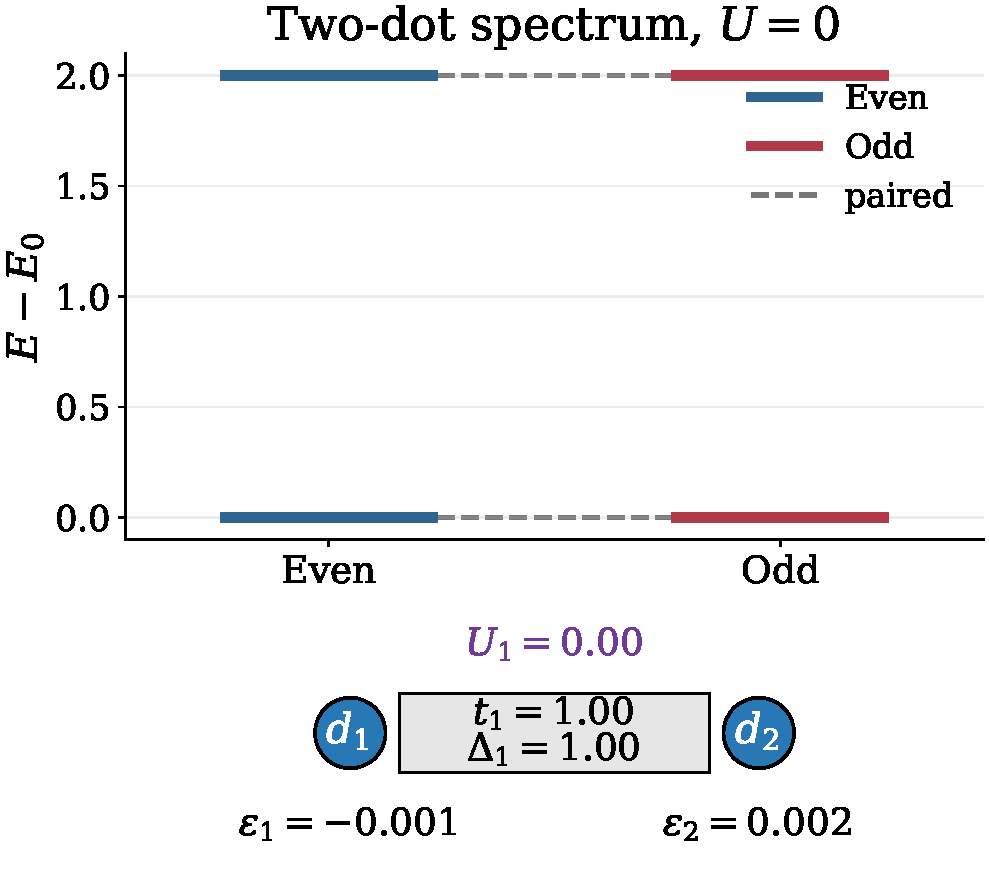
\includegraphics[width=0.49\textwidth]{figs/2DotU0.pdf}
  \hfill
  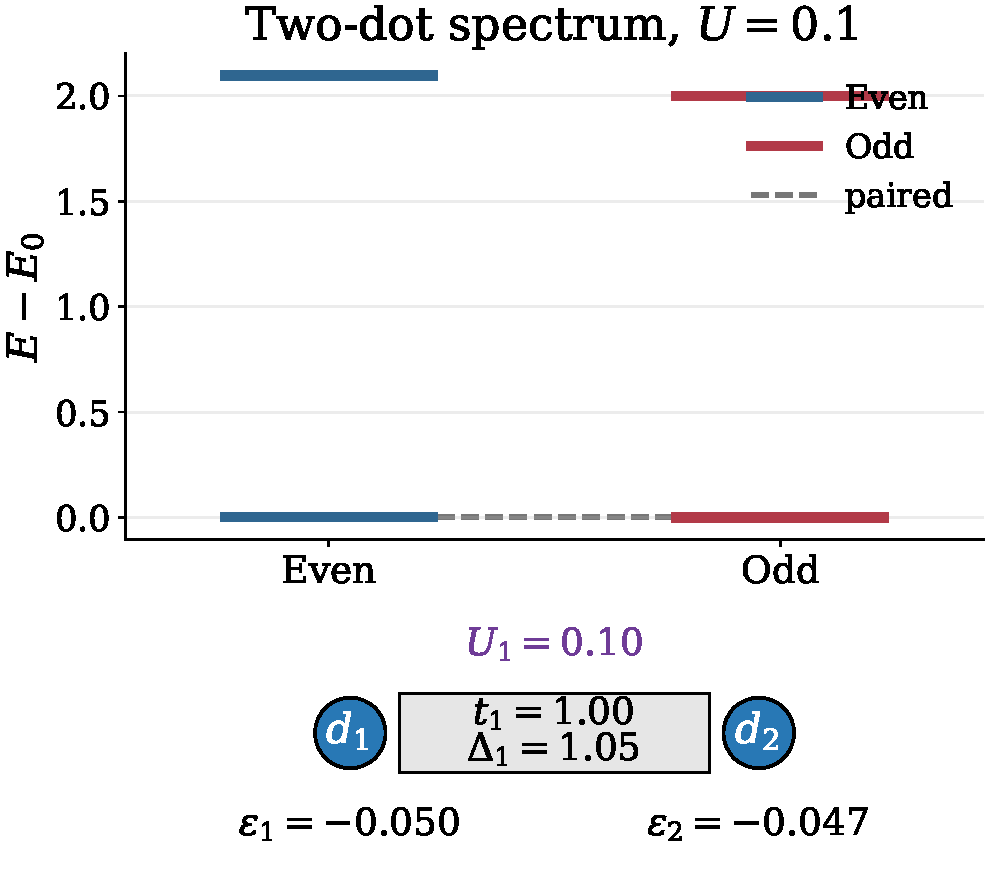
\includegraphics[width=0.49\textwidth]{figs/2DotU01.pdf}
  \caption{Parity-resolved spectra after optimization for the two-dot system at $U=0$ and $U=0.1$. Energies are shifted by the ground-state energy in each panel, and the optimized parameters are shown schematically below each spectrum.}
  \label{fig:2dot_schematicfirst}
\end{figure}

\begin{figure}[!htbp]
  \centering
  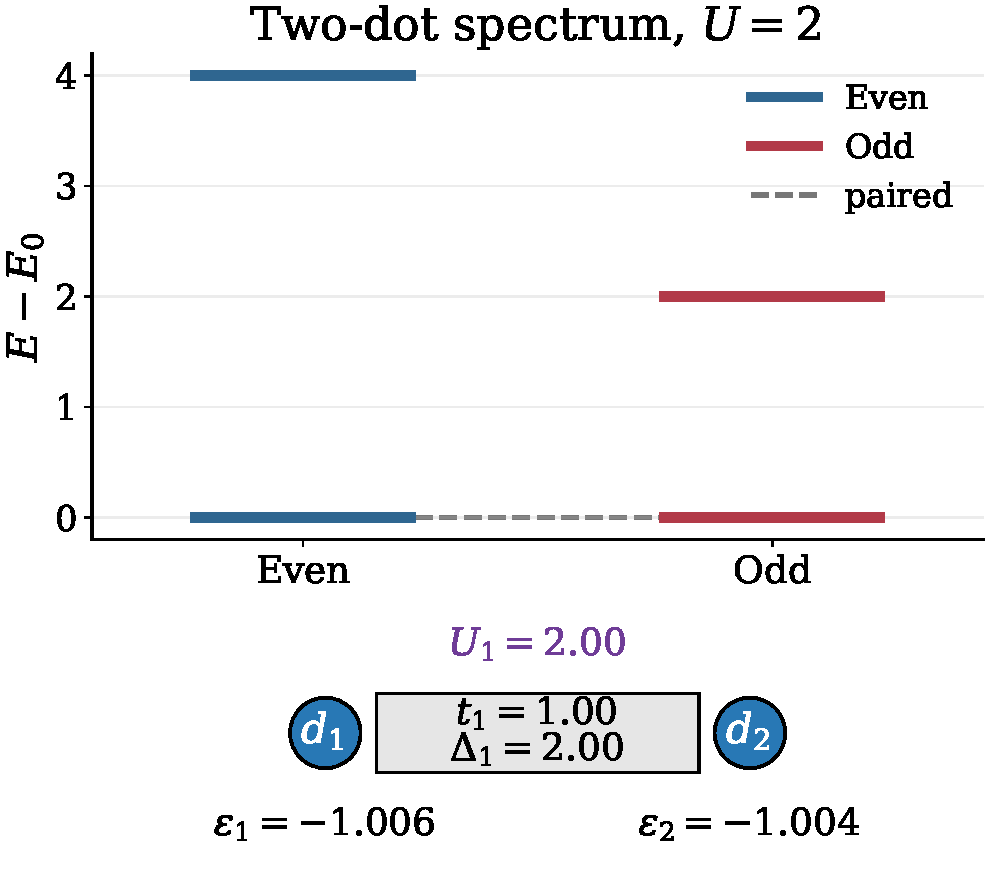
\includegraphics[width=0.74\textwidth]{figs/2DotU2.pdf}
  \caption{Parity-resolved spectrum after optimization for the two-dot system at $U=2.0$. Energies are shifted by the ground-state energy, and the optimized parameters are shown schematically below the spectrum.}
  \label{fig:2dot_schematicsecond}
\end{figure}
\newpage

The optimized three-dot system at $U=0.1$ provides a more promising
 configuration. As shown in Fig.~\ref{fig:3DotU01}, the
parity-resolved spectrum remains nearly paired, while the Majorana-polarization
profile has the expected edge-localized structure. The polarization is large
and opposite in sign on the two outer dots, and it is strongly suppressed on
the middle dot. This combination of spectral pairing and spatial Majorana
character motivates using this configuration as the main candidate for the
braiding calculations below. Comparing the three-dot and two-dot configurations at $U=0.1$ also illustrates how the additional site can help stabilize Majorana-like features in the presence of interactions. The excited-state degeneracy is better preserved in the three-dot case than in the two-dot case, even though both configurations have similar ground-state splitting and similar optimized parameters. The additional site therefore provides more freedom to optimize the excited states, which is important for maintaining a clean low-energy manifold that can support braiding.

\begin{figure}[!htbp]
  \centering
  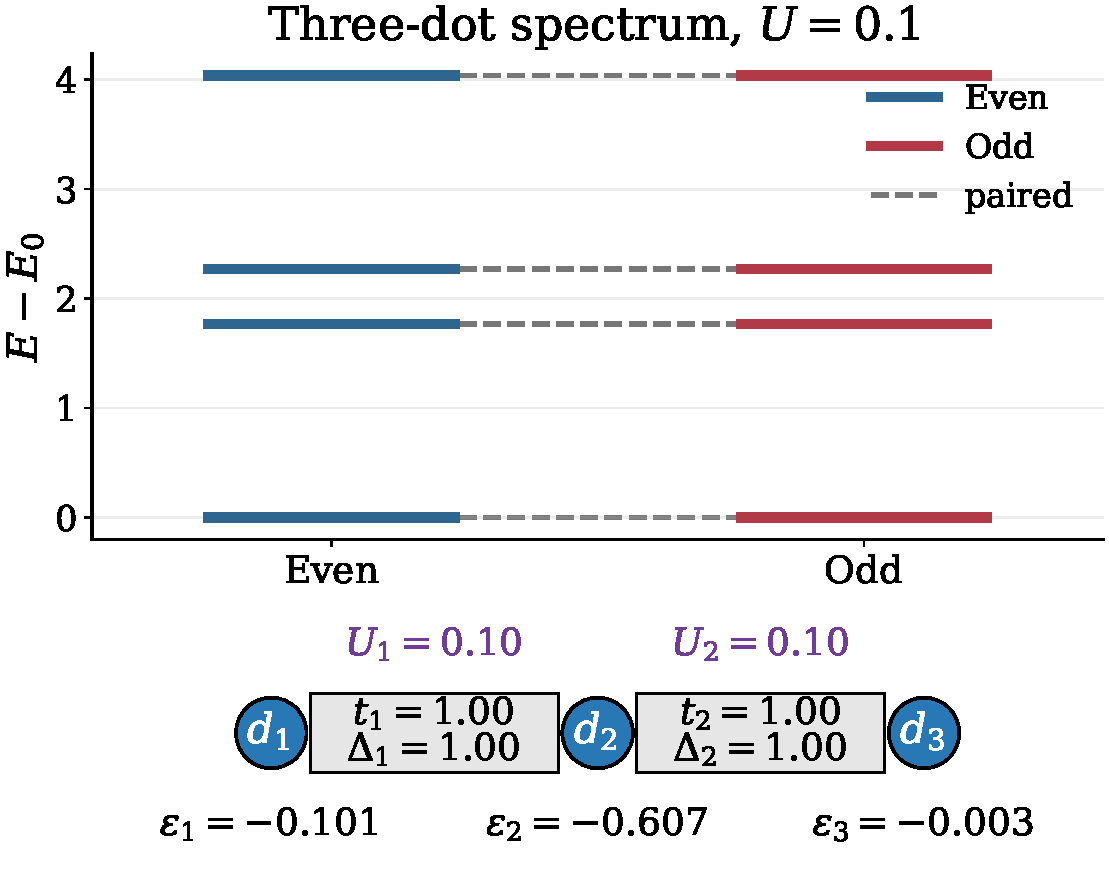
\includegraphics[width=0.55\textwidth]{figs/3DotU01.pdf}
  \hfill
  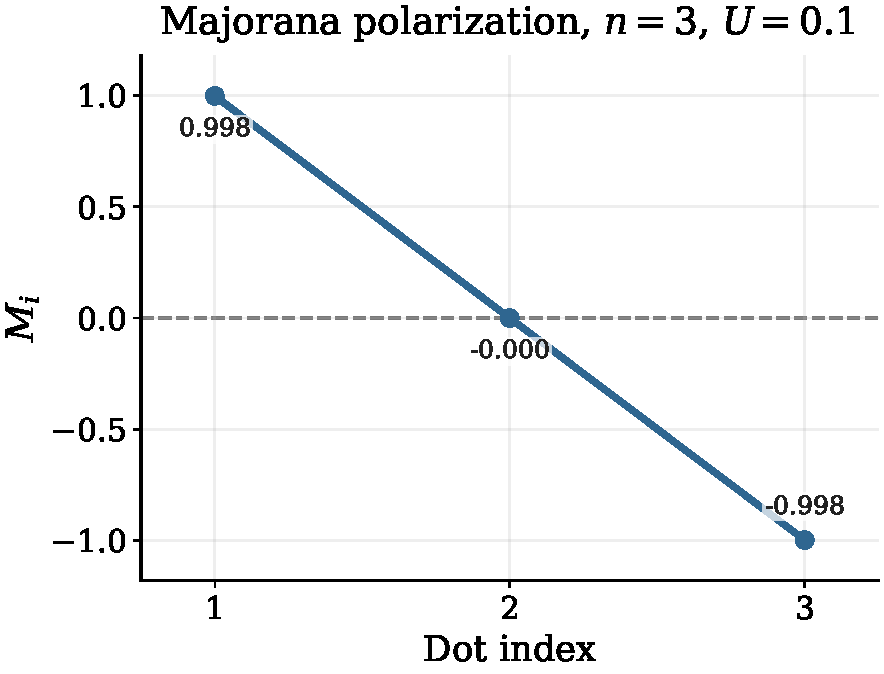
\includegraphics[width=0.41\textwidth]{figs/3DotMP01.pdf}
  \caption{Parity-resolved spectrum and Majorana-polarization profile for the optimized three-dot system at $U=0.1$. The left panel shows the optimized spectrum and parameters, while the right panel shows the Majorana polarization of the lowest even-odd pair.}
  \label{fig:3DotU01}
\end{figure}
\newpage

\section{Post-Optimization Diagnostics}
% The optimized parameter values alone do not determine whether a configuration is useful for Majorana braiding. 
After optimization, the candidate Hamiltonians must therefore be tested through spectral and local diagnostics. The parity-resolved spectra and low-energy gaps show whether the optimizer has produced an isolated nearly degenerate low-energy manifold, while the charge difference and Majorana-polarization profile test whether this manifold has the expected non-local and edge-localized Majorana character.

\subsection{Parity-resolved spectra and low-energy gaps}
\begin{figure}
  \centering
  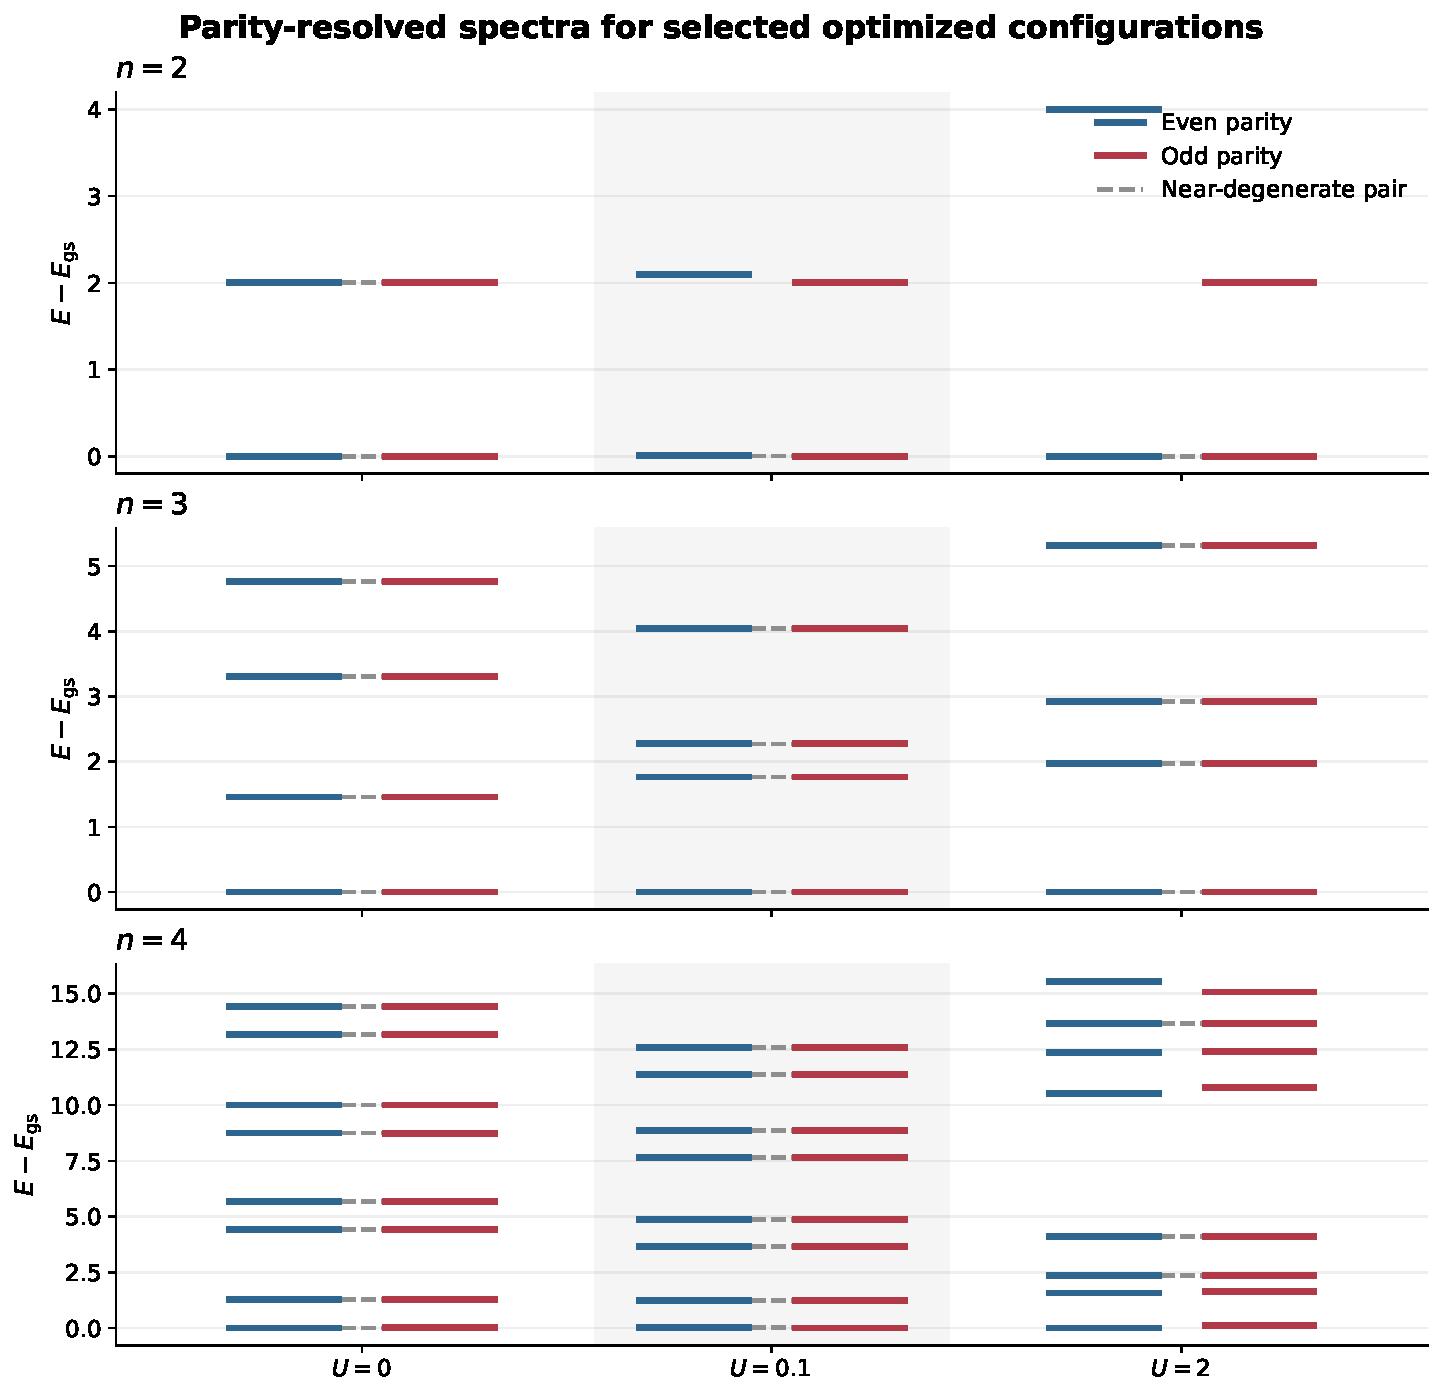
\includegraphics[width=\textwidth]{figs/parity_summary_u0_u01_u2.pdf}
  \caption{Parity-resolved spectra for the best optimized configurations at selected interaction strengths. Each panel corresponds to a different system size $n$, and energies are shifted so that the ground state is at zero.}
  \label{fig:parity_summary}
\end{figure}

Figure~\ref{fig:parity_summary} compares the parity-resolved spectra for $n=2,3,$ and $4$ at selected interaction strengths. A useful Majorana-like configuration should have a nearly degenerate lowest even-odd pair, together with a finite gap separating this pair from higher excited states. The dashed connectors in the figure indicate parity pairs that remain close in energy after optimization.

The non-interacting cases give the cleanest spectra, as expected. For the two-dot system, the parity pairing is nearly ideal at $U=0.0$, but the excited-state splitting becomes visible already at weak interaction and increases further at stronger interaction. 
% This shows that the interacting two-dot system can retain a low-energy degeneracy while losing clean parity pairing across the full finite spectrum.

The three-dot system is more stable across all interaction strengths shown, compared to both the two-dot and four-dot systems. For $U=0.0$, $U=0.1$, and $U=2.0$, the spectrum remains paired up to the numerical threshold, with relatively large gaps separating distinct energy sectors. The four-dot system shows a promising structure in the non-interacting and weakly interacting cases, while for the stronger interaction $U=2.0$ the energy degeneracy falls apart. Most importantly, the ground-state energies are no longer degenerate, so there is no longer a clear low-energy manifold that can support braiding. The three-dot system therefore appears to be the most robust candidate for maintaining a clean low-energy manifold across different interaction strengths, but the local diagnostics and Majorana character must also be checked before choosing it for braiding.

\subsection{Local diagnostics and Majorana character}
As discussed in the method chapter, Majorana-like states cannot be identified from spectral degeneracy alone. The parity-resolved spectra and low-energy gaps test whether the optimized Hamiltonian contains an isolated, nearly degenerate low-energy manifold. This subsection examines the complementary local diagnostics: the Majorana-polarization profile and the local charge difference between the lowest even-odd parity partners.

A convincing Majorana-like configuration should have opposite Majorana polarization on the two ends of the chain, with strongly suppressed polarization in the interior, as quantified by Eqs.~\ref{eq:method_edge_polarization} and~\ref{eq:method_bulk_polarization}. In addition, the even and odd parity partners should be locally difficult to distinguish. This is tested by the charge-difference diagnostic in Eq.~\ref{eq:method_charge_difference}, where smaller values indicate that the parity information is less visible to local charge measurements.

\begin{figure}[htbp]
  \centering
  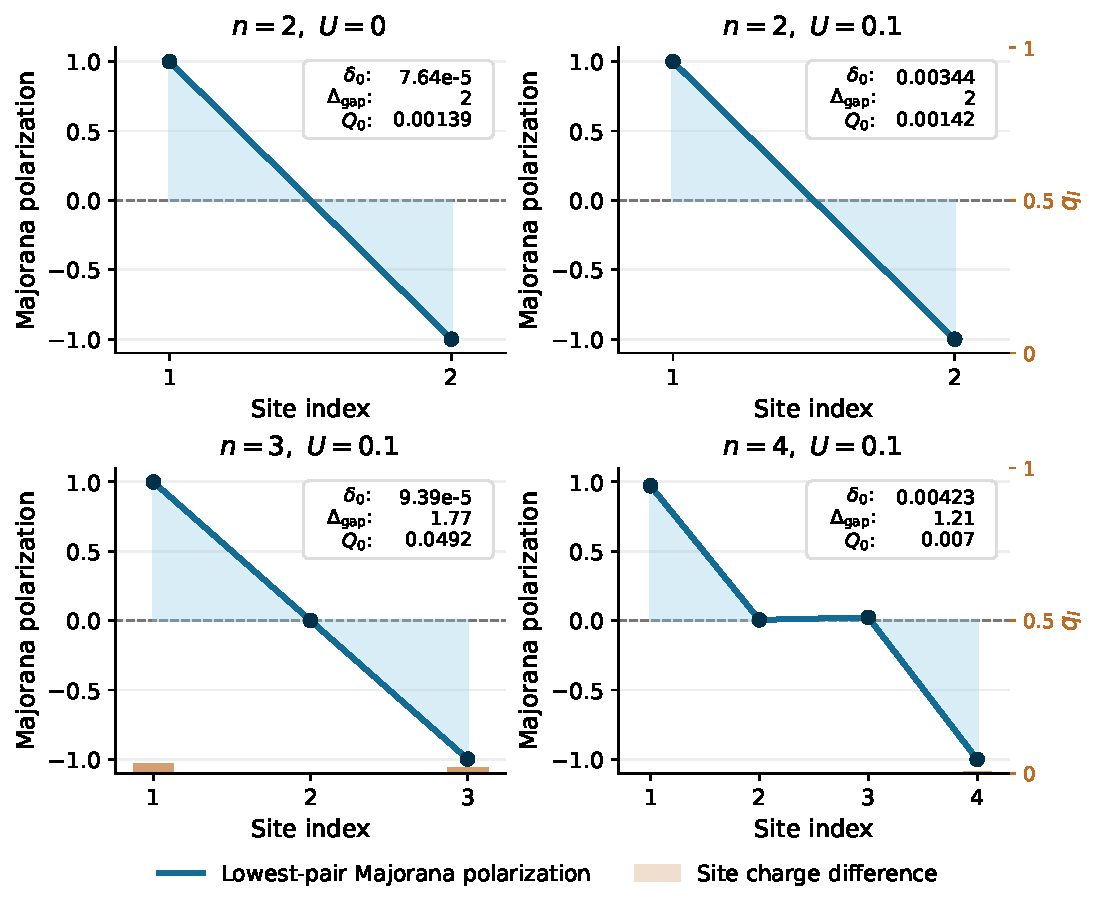
\includegraphics[width=0.95\textwidth]{figs/majorana_character_summary.pdf}
  \caption{Local diagnostics for representative optimized configurations. The blue curve shows the Majorana-polarization profile of the lowest even-odd pair, while the orange bars, read against the $0$--$1$ right axis, show the local charge difference $q_i=|\langle e | n_i | e \rangle - \langle o | n_i | o \rangle|$ on each site. The inset in each panel reports the ground-state splitting $\delta_0$, the low-energy gap $\Delta_{\mathrm{gap}}$, and the total charge difference $Q_0$.}
  \label{fig:majorana_character_summary}
\end{figure}
\newpage

\begin{table}
  \centering
  \begin{tabular}{c c c c c c c}
\hline
$n$ & $U$ & $\delta_0$ & $\Delta_{\mathrm{gap}}$ & $Q_0$ & $\overline{|M_{\mathrm{edge}}|}$ & $\max |M_{\mathrm{bulk}}|$ \\
\hline
2 & 0 & 7.64e-05 & 2 & 0.00139 & 1 & 0 \\
2 & 0.1 & 0.00344 & 2 & 0.00142 & 1 & 0 \\
3 & 0.1 & 9.39e-05 & 1.77 & 0.0492 & 0.998 & 0.000202 \\
4 & 0.1 & 0.00423 & 1.21 & 0.007 & 0.986 & 0.0233 \\
\hline
\end{tabular}

  \caption{Summary of local diagnostics for the representative configurations shown in Fig.~\ref{fig:majorana_character_summary}. Here $\delta_0$ is the splitting of the lowest even-odd pair, $\Delta_{\mathrm{gap}}$ is the gap separating this pair from the next excited states, $Q_0$ is the total charge difference between the parity partners, $\overline{|M_{\mathrm{edge}}|}$ is the mean absolute Majorana polarization on the first and last sites, and $\max |M_{\mathrm{bulk}}|$ is the largest absolute polarization on the interior sites.}
  \label{tab:majorana_character_summary}
\end{table}

Figure~\ref{fig:majorana_character_summary} compares the spatial profiles directly, while Table~\ref{tab:majorana_character_summary} summarizes the corresponding scalar diagnostics. For the two-dot system, the edge polarization is essentially ideal, with $\overline{|M_{\mathrm{edge}}|}\approx 1$ and no bulk contribution by construction. The total charge difference is also very small, $Q_0\approx 1.4\times 10^{-3}$, both at $U=0$ and at $U=0.1$. These two-dot cases are useful references, but because they have no interior sites they do not test suppression of Majorana weight in the bulk.

The three-dot configuration at $U=0.1$ gives the clearest interacting Majorana-polarization pattern. The ground-state splitting is only $\delta_0=9.39\times 10^{-5}$, the excitation gap remains large, $\Delta_{\mathrm{gap}}=1.77$, and the bulk polarization is almost completely suppressed, with $\max |M_{\mathrm{bulk}}|=2.02\times 10^{-4}$. Its charge difference, however, is larger than in the two-dot and four-dot reference cases, with $Q_0=0.0492$. This shows that the three-dot state is not ideal in every diagnostic, even though its spectral and polarization properties are the strongest.

The four-dot configuration at $U=0.1$ shows the opposite tradeoff. It has a smaller charge difference, $Q_0=0.0070$, and comparably strong edge polarization, $\overline{|M_{\mathrm{edge}}|}\approx 0.986$. However, the ground-state splitting increases to $\delta_0=4.23\times 10^{-3}$ and the bulk polarization rises to $\max |M_{\mathrm{bulk}}|=2.33\times 10^{-2}$.

Together, these diagnostics show that different system sizes optimize different aspects of the Majorana criteria. The four-dot case performs better in terms of local charge indistinguishability, while the three-dot case performs better in terms of spectral near-degeneracy and suppression of bulk Majorana weight. Since the braiding analysis requires a low-energy subspace that is both nearly degenerate and spatially well localized, the interacting three-dot system remains the most convincing candidate for the rest of the thesis.

\section{Selection of Braiding Candidate}
The braiding calculations are performed using the optimized three-dot configuration at $U=0.1$. This choice is based on the combined post-optimization diagnostics above. Although the four-dot configuration has a smaller local charge difference, the three-dot configuration has the most favorable combination of small ground-state splitting, large excitation gap, clear edge-localized Majorana-polarization profile, and strongly suppressed bulk polarization. Since the braiding analysis relies on a nearly degenerate and spatially localized low-energy subspace, the three-dot system is chosen as the main microscopic building block.

The optimized parameters used for each three-dot subsystem are
\begin{equation}
\Delta_1=1.001,\qquad
\Delta_2=1.002,\qquad
\epsilon_1=-0.101,\qquad
\epsilon_2=-0.607,\qquad
\epsilon_3=-0.003,
\end{equation}
with fixed hopping amplitudes $t_i=1$ and fixed interaction strength $U=0.1$.
 
In the braiding geometry, three identical copies of this optimized three-dot chain are combined. Each subsystem has Hilbert-space dimension $2^3=8$, giving a total microscopic Hilbert space of dimension $2^9=512$. This system is large enough to test braiding beyond the lowest projected manifold, while still being small enough for exact diagonalization and systematic sector-resolved scans. The selected configuration therefore provides a useful setting for studying how interactions affect braiding across the many-body spectrum.

\section{Braiding in the Ground-State Sector}
The optimized three-dot chain is now used as the building block for the braiding calculations. Before studying higher energy sectors, we first establish a controlled ground-state benchmark. The goal is to separate three related questions: whether the energy-level Majorana operators generate the expected exchange, whether projected microscopic junction couplings select the same exchange channel, and whether this channel is also visible through projected local endpoint operators.

The energy-level reference model generates the braid directly from tunable Majorana bilinears built from the four Majorana operators defined in Eq.~\ref{eq:four_majoranas}. This provides the clean baseline for the exchange protocol. In the projected microscopic junction model, these direct bilinears are replaced by projected junction operators constructed from the hopping and crossed-Andreev pairing Hamiltonian introduced in Eq.~\ref{eq:junctionHamiltonian}. After projection into the retained low-energy subspace, this gives the effective couplings \(T_{AB}\) and \(T_{AC}\) defined in Eq.~\ref{eq:method_projected_junctions}, which are used in the driven braid Hamiltonian of Eq.~\ref{eq:brajunc}. Finally, the projected local-operator model uses endpoint Majorana components instead of the full junction Hamiltonian, testing whether the same low-energy exchange channel is accessed by local microscopic operators.



\subsection{Energy-Level Majorana Reference}
\begin{figure}[htbp]
  \centering
  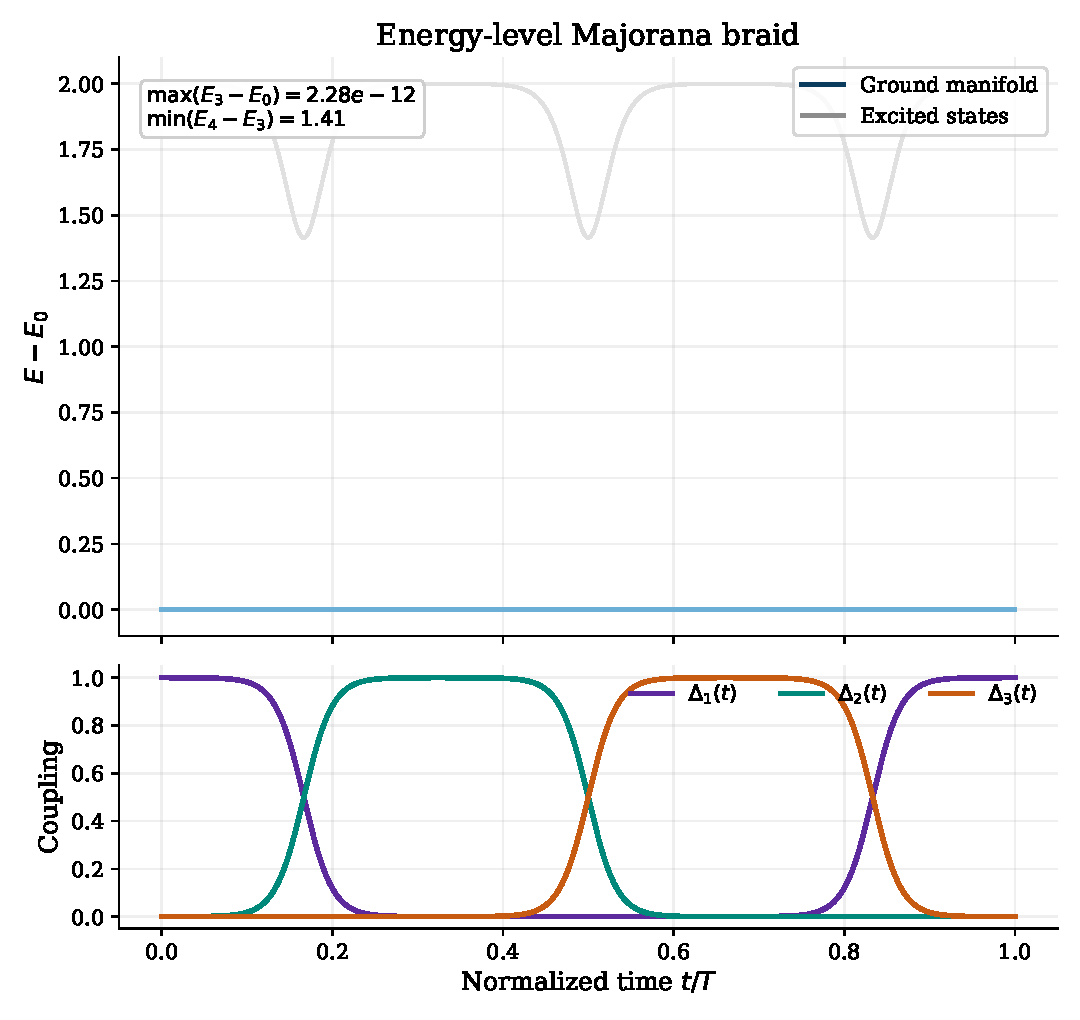
\includegraphics[width=0.9\textwidth]{figs/braiding_ideal_protocol.pdf}
  \caption{Energy-level Majorana braiding protocol. The top panel shows the instantaneous spectrum of the effective Hamiltonian during the braid, with all energies shifted so that the lowest state remains at zero. The bottom panel shows the three smooth pulse couplings that move the dominant Majorana coupling through the network.}
  \label{fig:braiding_ideal_protocol}
\end{figure}

Figure~\ref{fig:braiding_ideal_protocol} shows the reference braid generated by four active Majorana operators in the projected low-energy space. The three couplings are turned on sequentially, so that the dominant coupling is first between $\gamma_0$ and $\gamma_1$, then between $\gamma_0$ and $\gamma_2$, and finally between $\gamma_0$ and $\gamma_3$ before returning to the initial configuration. Throughout this cycle, the transported low-energy manifold remains essentially four-fold degenerate. The largest instantaneous splitting within this manifold is only $\max(E_3-E_0)=2.28\times 10^{-12}$, while the minimum gap to the excited states remains open at $\min(E_4-E_3)=1.414$.

Using Kato transport, the resulting unitary reproduces the expected single-exchange action on the Majorana operators. The largest error in the transformations $\gamma_2\rightarrow-\gamma_3$ and $\gamma_3\rightarrow\gamma_2$ is $3.34\times 10^{-6}$. In the parity-resolved gate blocks, the odd and even $2\times2$ blocks agree with the target exchange gate to within $6.53\times 10^{-8}$, while the off-block leakage is only $1.02\times 10^{-11}$. The effective model therefore provides a clean benchmark for the more microscopic projected calculations.

\newpage
\subsection{Projected Microscopic Junction Braid}
In this subsection we replace the direct Majorana-bilinear couplings from the previous subsection with the projected microscopic junction operators defined in Eq.~\ref{eq:method_projected_junctions}. The goal is to test whether it is possible to reproduce the same low-energy exchange channel using the junction Hamiltonian of Eq.~\ref{eq:junctionHamiltonian} instead of direct Majorana bilinears. This subsection identifies two separate findings. The first is which Majorana operators are actually being exchanged in the microscopic model. The second is whether this junction-based exchange can reproduce the target exchange channel of the energy-level reference model. 
\begin{figure}[htbp]
  \centering
  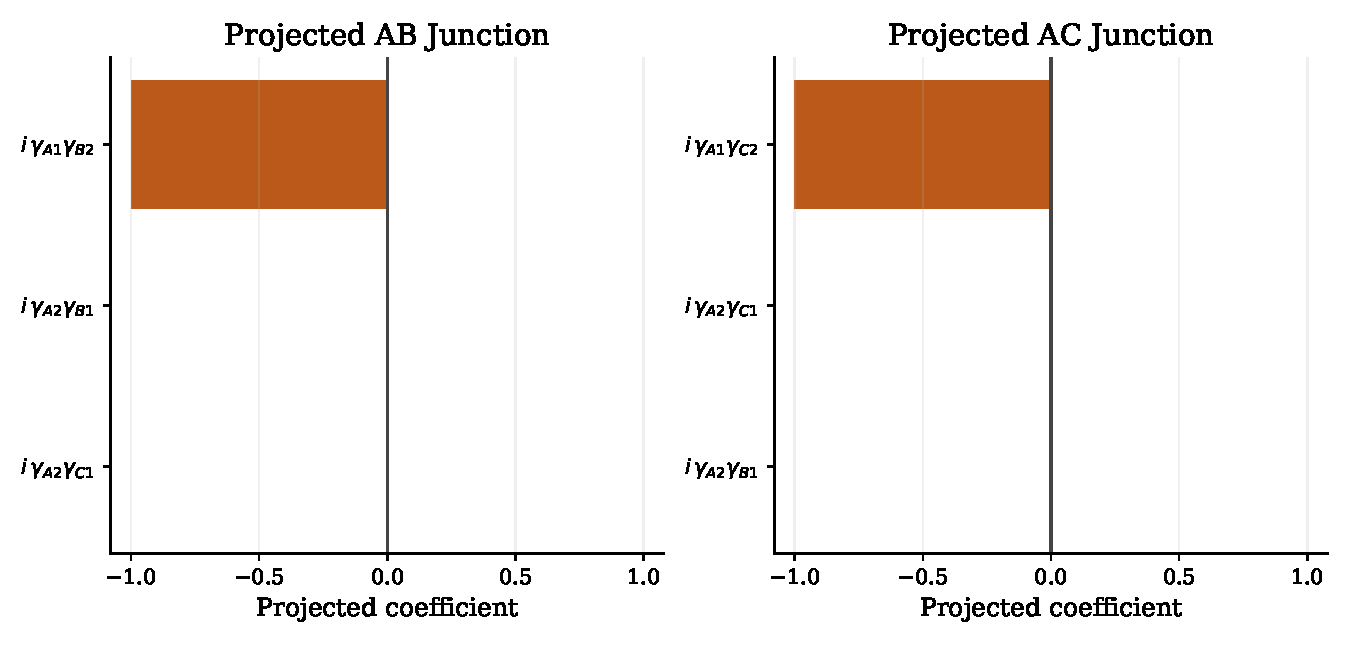
\includegraphics[width=0.95\textwidth]{figs/braiding_junction_decomposition.pdf}
  \caption{Dominant Majorana-bilinear components of the projected microscopic junction operators. The AB junction is almost entirely $i\gamma_{A1}\gamma_{B2}$, while the AC junction is almost entirely $i\gamma_{A1}\gamma_{C2}$. All subleading bilinears are strongly suppressed.}
  \label{fig:braiding_junction_decomposition}
\end{figure}

\Cref{fig:braiding_junction_decomposition} shows the decomposition of the projected junction terms $T_{AB}$ and $T_{AC}$ in the energy-level Majorana-bilinear basis. The AB junction is dominated by the bilinear $i\gamma_{A1}\gamma_{B2}$, while the AC junction is dominated by $i\gamma_{A1}\gamma_{C2}$. This identifies $\gamma_{B2}$ and $\gamma_{C2}$ as the Majoranas that participate in the microscopic braid, while $\gamma_{A1}$ acts as the shared Majorana through which the exchange is mediated. The remaining bilinear components are strongly suppressed, indicating that the junction Hamiltonian effectively selects a single low-energy exchange channel.  

\begin{figure}[htbp]
  \centering
  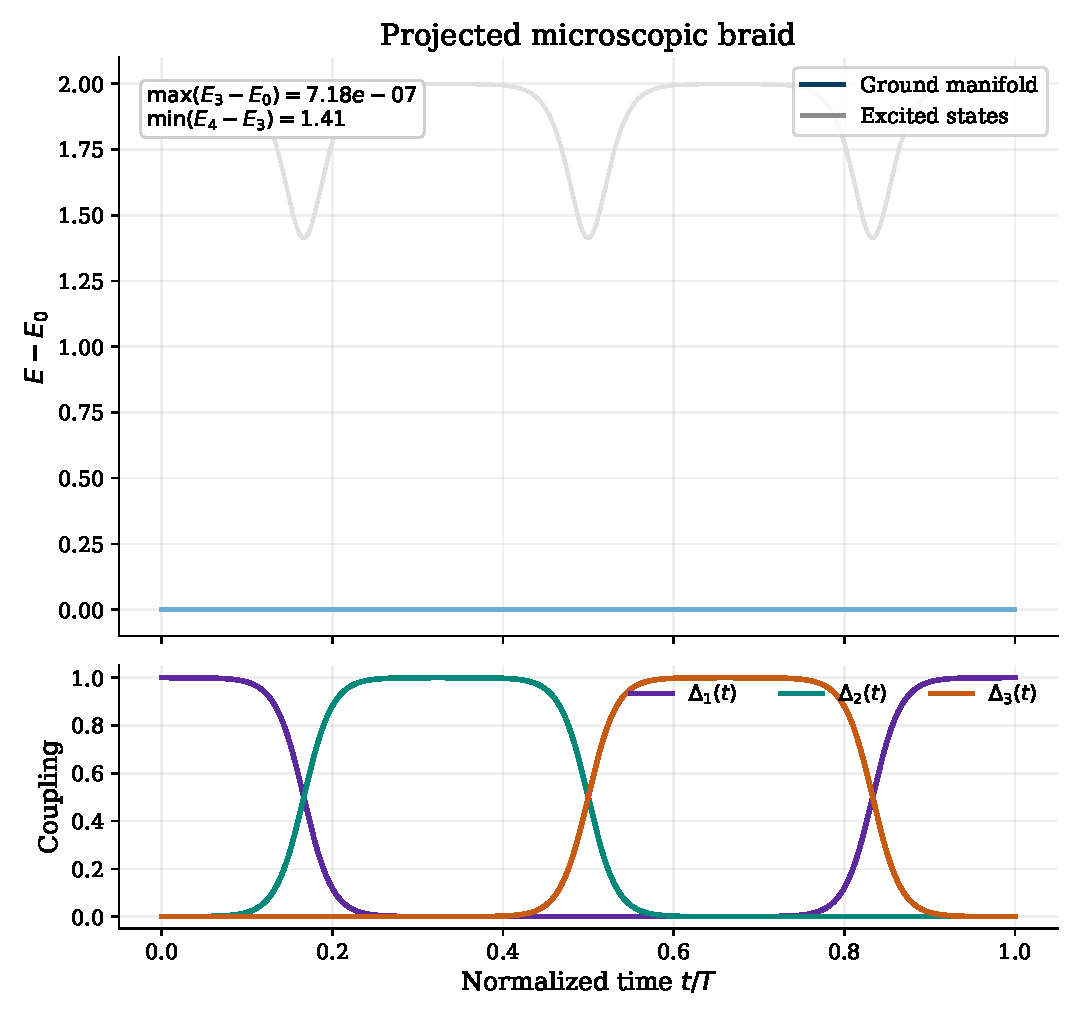
\includegraphics[width=0.9\textwidth]{figs/braiding_projected_protocol.pdf}
  \caption{Braiding protocol after replacing the direct reference couplings by projected microscopic junction operators. The spectral evolution remains almost identical to the energy-level benchmark, with a well-isolated low-energy manifold throughout the cycle.}
  \label{fig:braiding_junctionprotocol}
\end{figure}
\Cref{fig:braiding_junctionprotocol} shows the resulting braid after replacing the energy-level Majorana bilinears with the projected microscopic junction operators. The spectral evolution remains almost identical to the effective-model benchmark, with a well-isolated low-energy manifold throughout the cycle. The maximum splitting inside this manifold increases only to $\max(E_3-E_0)=7.18\times 10^{-7}$, while the minimum gap remains large, $\min(E_4-E_3)=1.413$.

\newpage
\subsection{Projected Local-Operator Braid}
The junction decomposition above identifies $\gamma_{B2}$ and $\gamma_{C2}$ as the active exchange channels. The next question is whether the same channels are obtained from local endpoint Majorana operators. For this, we use the projected local component
\[
\Gamma_{S,-}^{P}
=
\mathcal{N}_S V^\dagger \chi_{S,-}V,
\qquad
\chi_{S,-}=i(c_S^\dagger-c_S),
\]
corresponding to the \(\Gamma_-^P\) component introduced in Eq.~\ref{eq:local_gamma_ops}. The local-operator braid is then generated with the Hamiltonian of Eq.~\ref{eq:local_braid_ham}, using the same pulse sequence as in the energy-level and projected microscopic junction models.

\begin{table}[htbp]
  \centering
  \begin{tabular}{lcc}
\hline
Projected local operator & Dominant energy-level Majorana & Coefficient \\
\hline
$\Gamma_{B,\mathrm{L},-}^{P}$ & $\gamma_{B2}$ & -1.000 \\
$\Gamma_{B,\mathrm{R},-}^{P}$ & $\gamma_{B2}$ & 1.000 \\
$\Gamma_{C,\mathrm{L},-}^{P}$ & $\gamma_{C2}$ & -1.000 \\
$\Gamma_{C,\mathrm{R},-}^{P}$ & $\gamma_{C2}$ & 1.000 \\
\hline
\multicolumn{3}{l}{Endpoint consistency checks} \\
\hline
$B$ endpoints, $\chi_-$ component & opposite orientation & 8.969e-14 \\
$C$ endpoints, $\chi_-$ component & opposite orientation & 5.787e-14 \\
\hline
\end{tabular}

  \caption{Projected local endpoint operators used in the local-operator braid. The minus components project onto the same low-energy Majorana channels selected by the microscopic junction decomposition, $\gamma_{B2}$ and $\gamma_{C2}$, up to endpoint orientation.}
  \label{tab:braiding_local_projection}
\end{table}

\Cref{tab:braiding_local_projection} shows that the projected local minus components on the relevant endpoint sites select the same low-energy channels as the projected junction calculation. The left and right endpoint projections in subsystem $B$ both reduce to $\gamma_{B2}$, but with opposite orientation, and the same happens for subsystem $C$ and $\gamma_{C2}$. This sign only fixes the endpoint convention for the projected operator; the factor of $i$ is already contained in the definition of the minus component $\chi_-=i(c^\dagger-c)$.

\begin{figure}[htbp]
  \centering
  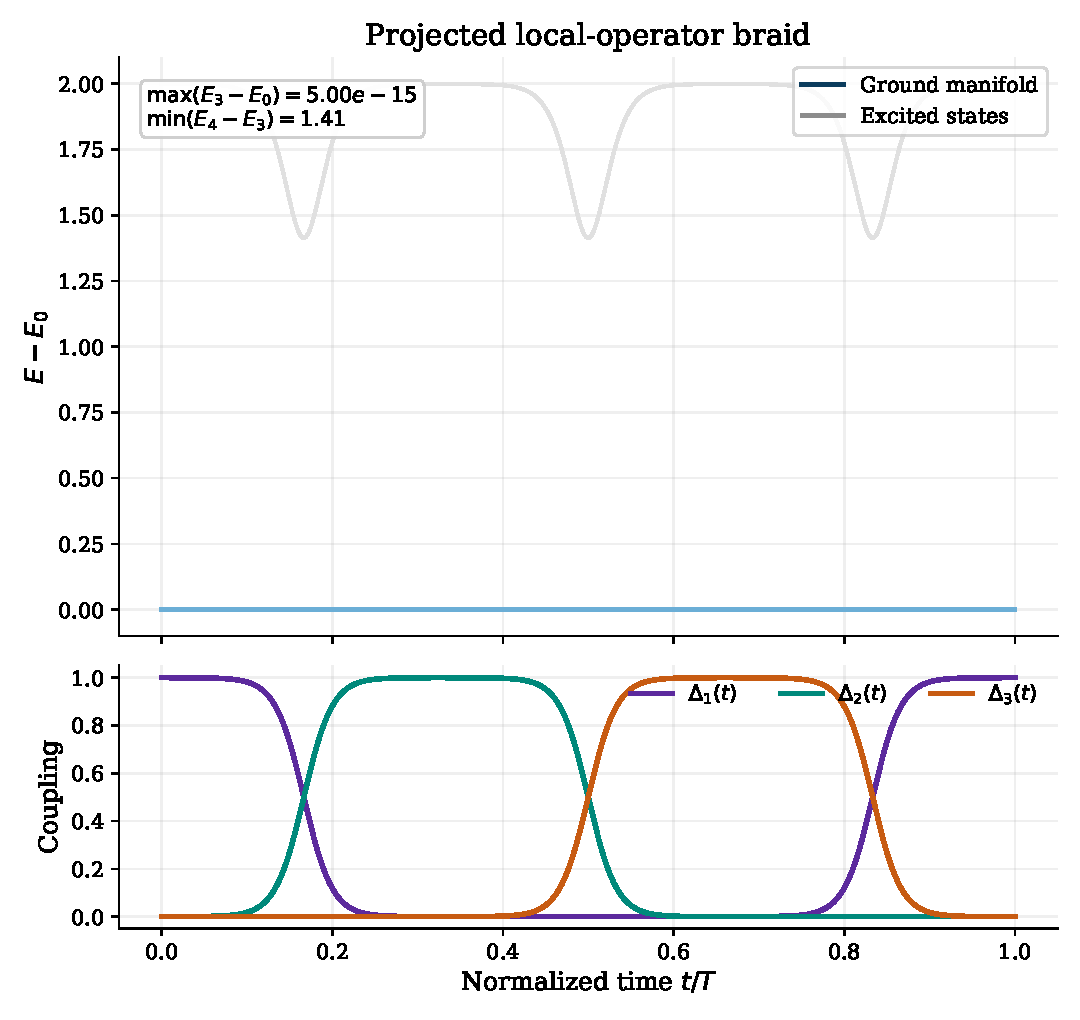
\includegraphics[width=0.9\textwidth]{figs/braiding_local_operator_protocol.pdf}
  \caption{Projected local-operator braiding protocol. The driven couplings follow the same pulse sequence as in the energy-level and projected microscopic junction models, but the exchanged operators are constructed from projected local endpoint Majorana components.}
  \label{fig:braiding_local_operator_protocol}
\end{figure}

\Cref{fig:braiding_local_operator_protocol} shows that the projected local-operator braid has the same stable low-energy structure as the two previous ground-sector braids. The transported four-dimensional manifold remains essentially degenerate, with $\max(E_3-E_0)=5.00\times10^{-15}$, while the gap to the excited states remains open at $\min(E_4-E_3)=1.414$.

\begin{table}[htbp]
  \centering
  \setlength{\tabcolsep}{5pt}
  \begin{tabular}{lcccccc}
\hline
Model & Split & Gap & 1x err. & Leakage & Odd err. & Even err. \\
\hline
Energy-level & 2.275e-12 & 1.414 & 3.343e-06 & 1.016e-11 & 6.527e-08 & 6.527e-08 \\
Projected junction & 7.175e-07 & 1.413 & 3.343e-06 & 8.727e-16 & 6.531e-08 & 6.531e-08 \\
Projected local & 4.996e-15 & 1.414 & 3.343e-06 & 7.542e-16 & 6.530e-08 & 6.530e-08 \\
\hline
\end{tabular}

  \caption{Comparison of the main braid diagnostics for the energy-level Majorana reference model, the projected microscopic junction model, and the projected local-operator model. Here ``Split'' denotes $\max(E_3-E_0)$, ``Gap'' denotes $\min(E_4-E_3)$, ``1x err.'' is the largest deviation in the expected single-exchange Majorana map, ``Leakage'' is the off-block norm in the parity basis, and the last two columns compare the odd and even parity blocks with the target exchange gate.}
  \label{tab:braiding_checks_comparison}
\end{table}

\Cref{tab:braiding_checks_comparison} shows that all three ground-sector braid constructions give essentially the same result. The maximum single-exchange error is $3.34\times10^{-6}$ in each case, the parity leakage remains below $10^{-11}$, and the odd- and even-parity blocks agree with the target exchange gate to approximately $6.5\times10^{-8}$. In the ground-state sector, the projected local endpoint operators therefore access the same exchange channel as the energy-level and microscopic junction constructions.

\newpage
\section{Braiding in Multiple Energy Sectors}
To explore whether braiding is possible beyond the lowest projected manifold, we first identify distinct energy sectors in the three-dot, three-subsystem system. This is done by combining the three single-subsystem Hamiltonians into one full-system Hamiltonian,
\begin{equation}
  H = H_A \otimes I_B \otimes I_C
  + I_A \otimes H_B \otimes I_C
  + I_A \otimes I_B \otimes H_C .
\end{equation}
This Hamiltonian captures the entire $2^9 \times 2^9$ Hilbert space of the Y-junction system. The three subsystems, $A$, $B$, and $C$, are initially decoupled and identical.

The full-system spectrum can then be grouped into distinct energy sectors. Each sector consists of states that are degenerate in energy, within the numerical tolerance, and separated by a gap from neighboring sectors, as shown in \cref{fig:full_hamil_elevels}.

\begin{figure}[htbp]
  \centering
  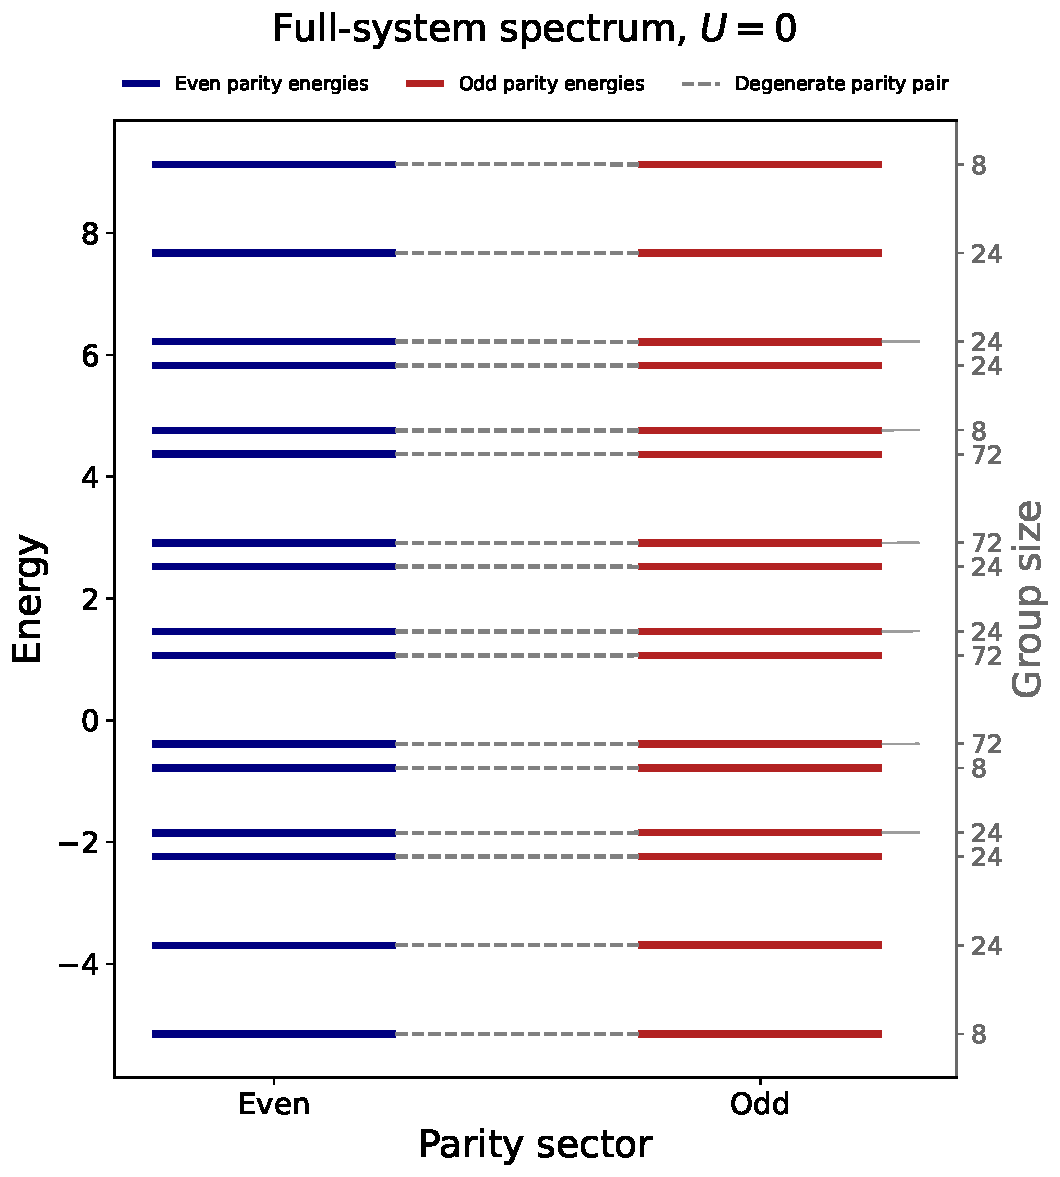
\includegraphics[width=0.9\textwidth]{figs/full_system_spectrum_U_0p0.pdf}
  \caption{Full-system Hamiltonian energy spectrum. The spectrum is split into even and odd eigenenergies. The dashed lines represent the degeneracy link between the even and odd sectors. The left-hand y-axis shows the energy levels, while the right-hand y-axis shows how many states reside in each energy sector. This figure was created for a single non-interacting system. Similar plots for the interacting model can be found in Appendix~\ref{app:energy_sectors}.}
  \label{fig:full_hamil_elevels}
\end{figure}

After the sectors have been identified, the same braid protocol can be applied sector by sector. For sector $i$, we form a sector basis $V_i$ from the eigenvectors belonging to that sector, and operators are represented in the selected space as $V_i^\dagger O V_i$, as described in \cref{eq:method_operator_projection}. This makes it possible to test whether each braid construction produces its intended exchange behavior beyond the lowest projected manifold.

The sector bases have different dimensions. For example, the ground-state sector contains $8$ states inside the full $512$-dimensional Hilbert space, while the first excited sector contains $24$ states. When the braid couplings are activated, the selected sector splits into a lower and an upper band of equal dimension, separated by a gap, as shown in \cref{fig:level_split}. This split provides a well-defined lower band for Kato transport, but does not by itself establish that the resulting unitary performs a successful Majorana exchange. The target-overlap deviation \(D_{\mathcal{O}}=|1-\mathcal{O}|\), defined in \cref{eq:method_overlap_deviation}, provides that separate test.

For the sector-resolved scans, the transported dimension was therefore fixed to half of the selected sector dimension, as defined in \cref{eq:method_sector_transport_dimension}. In each sector, the Kato calculation transports the lower band and measures whether its final unitary reproduces the intended exchange. The scans below are self-target comparisons: each braid construction is compared with its own target operator. Agreement between the projected local and energy-level exchange channels requires the separate common-target comparison discussed in the method section.

\begin{figure}[htbp]
  \centering
  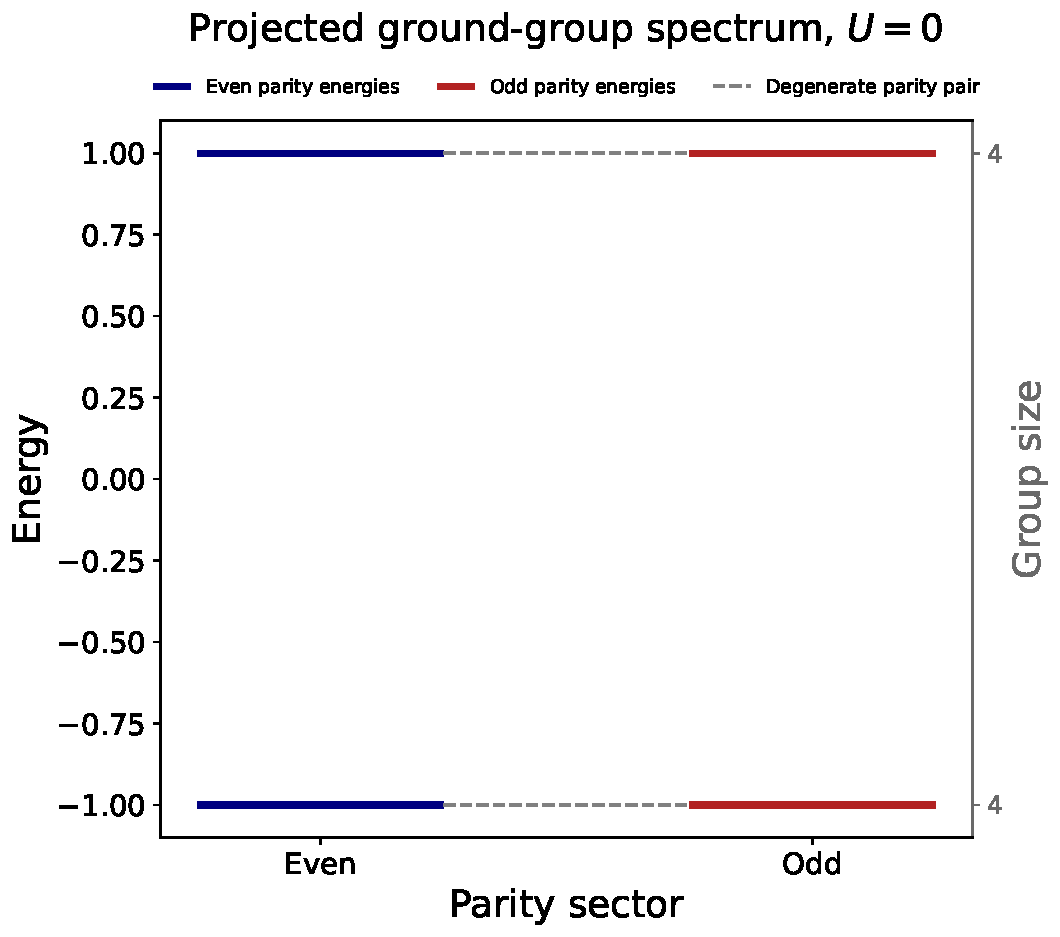
\includegraphics[width=0.9\textwidth]{figs/projected_ground_group_spectrum_U_0p0.pdf}
  \caption{Splitting of an initially degenerate energy sector into two distinct bands when the braid Hamiltonian is initialized. This representative example is the ground-state sector of the projected local-operator braid in the non-interacting system.}
  \label{fig:level_split}
\end{figure}



The first scan provides an energy-level Majorana baseline, starting with the ground-state sector and then moving through the higher energy sectors while simultaneously checking different interaction strengths. In this construction, the Majorana operators are built directly from paired even and odd eigenstates of each optimized subsystem. The non-interacting case provides the cleanest reference, while the interacting cases test whether the energy-level exchange channel extracted from the optimized spectra remains stable across sectors.
\begin{figure}[htbp]
  \centering
  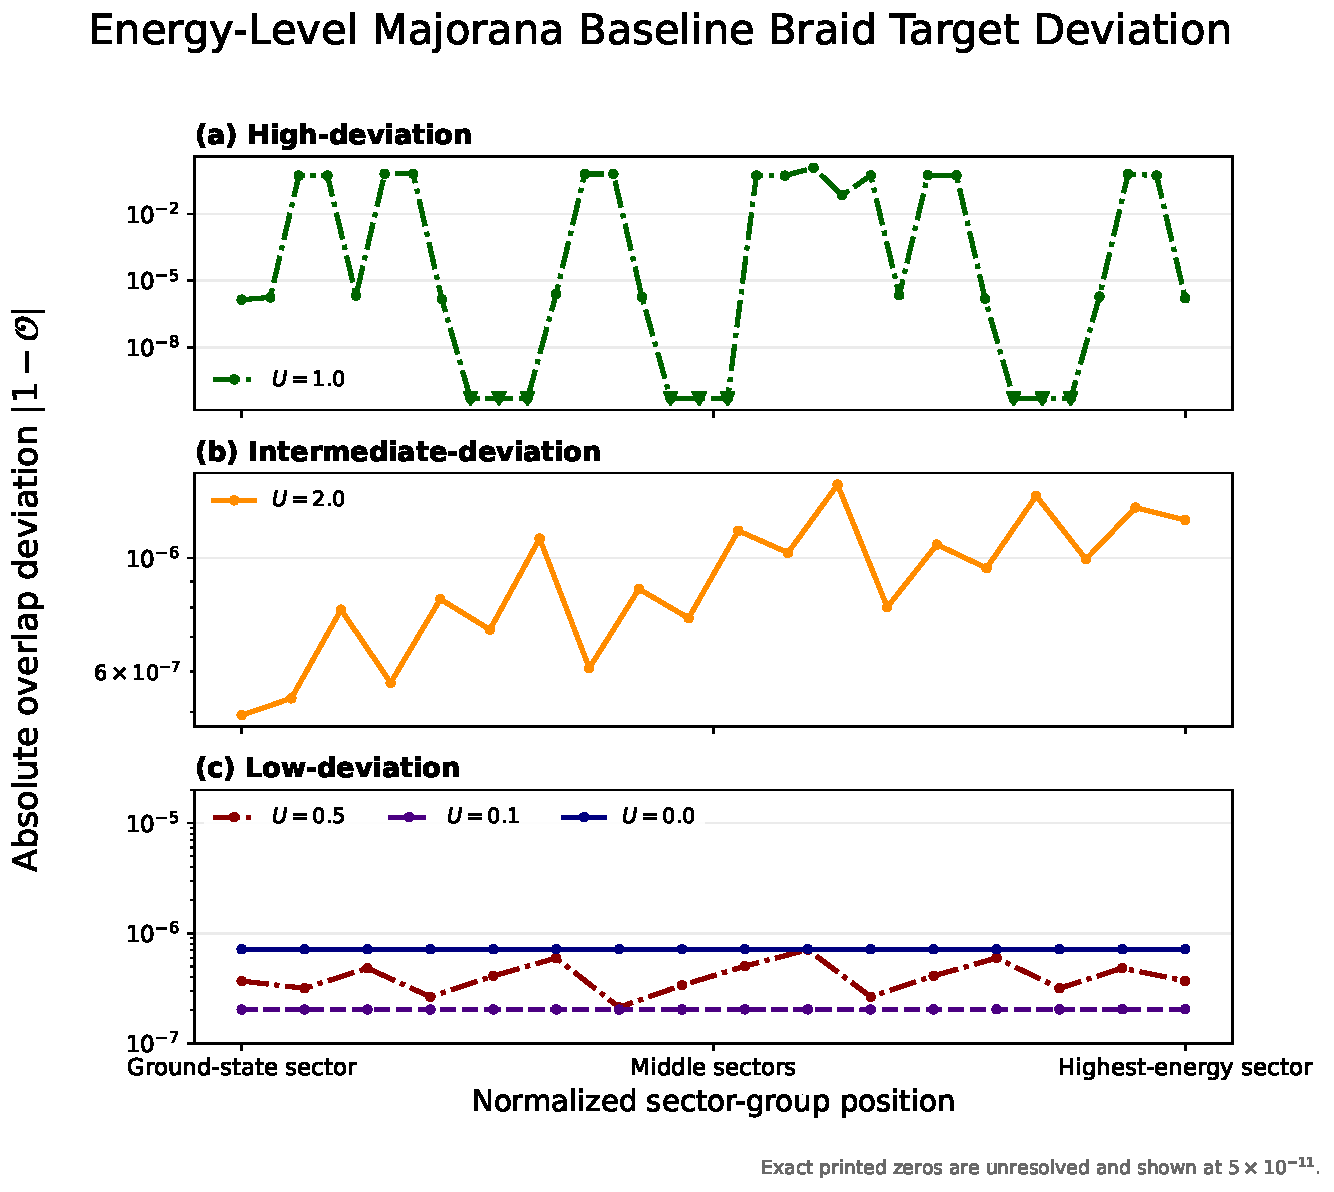
\includegraphics[width=0.9\textwidth]{figs/ideal_operator_interaction_regimes.pdf}
  \caption{Self-target braid errors for the energy-level Majorana baseline across different energy sectors and interaction strengths $U=0.0$, $U=0.1$, $U=0.5$, $U=1.0$, and $U=2.0$, plotted as the overlap deviation \(D_{\mathcal{O}}=|1-\mathcal{O}|\). The figure is split into three deviation regimes: a) $U=1.0$, b) $U=2.0$, and c) $U=0.0$, $U=0.1$, and $U=0.5$. The energy-level construction supports accurate braiding across all sectors for the non-interacting and weakly interacting configurations, while the $U=1.0$ configuration shows strong sector-dependent failures.}
  \label{fig:ideal_operator_interaction_regimes}
\end{figure}
\newpage
\Cref{fig:ideal_operator_interaction_regimes} displays the energy-level Majorana baseline. Here the $\gamma$ operators are created directly from the paired eigenstates by the construction $\gamma=\ket{e}\bra{o}+\mathrm{h.c.}$ before being projected into each sector and placed in the braid Hamiltonian. The high-deviation panel shows that the $U=1.0$ configuration is strongly sector dependent, as some sectors remain accurate, while others have errors of order $10^{-1}$. The $U=2.0$ results are much more stable across sectors and generally lie around $10^{-6}$. For $U=0.0$, $U=0.1$, and $U=0.5$, the errors remain below the $10^{-6}$ threshold across all sectors. The unusually poor and irregular $U=1.0$ result, despite the stronger $U=2.0$ configuration performing better in this baseline, shows that interaction strength alone does not necessarily explain the ordering of the selected configurations.



Since the low-energy junction decomposition identifies $\gamma_{B2}$ and $\gamma_{C2}$ as the active exchange channels, the projected local-operator model uses the minus endpoint components in subsystems $B$ and $C$,
\begin{equation}
  \Gamma_{S,-}^{(i)}
  =
  \mathcal{N}_{S,i}V_i^\dagger \chi_{S,-}V_i,
  \qquad
  \chi_{S,-}=i(c_S^\dagger-c_S),
  \qquad
  S=B,C.
\end{equation}
When these local operators are compared with $\gamma_{B2}$ and $\gamma_{C2}$, only an overall plus or minus sign is allowed.

\begin{figure}[htbp]
  \centering
  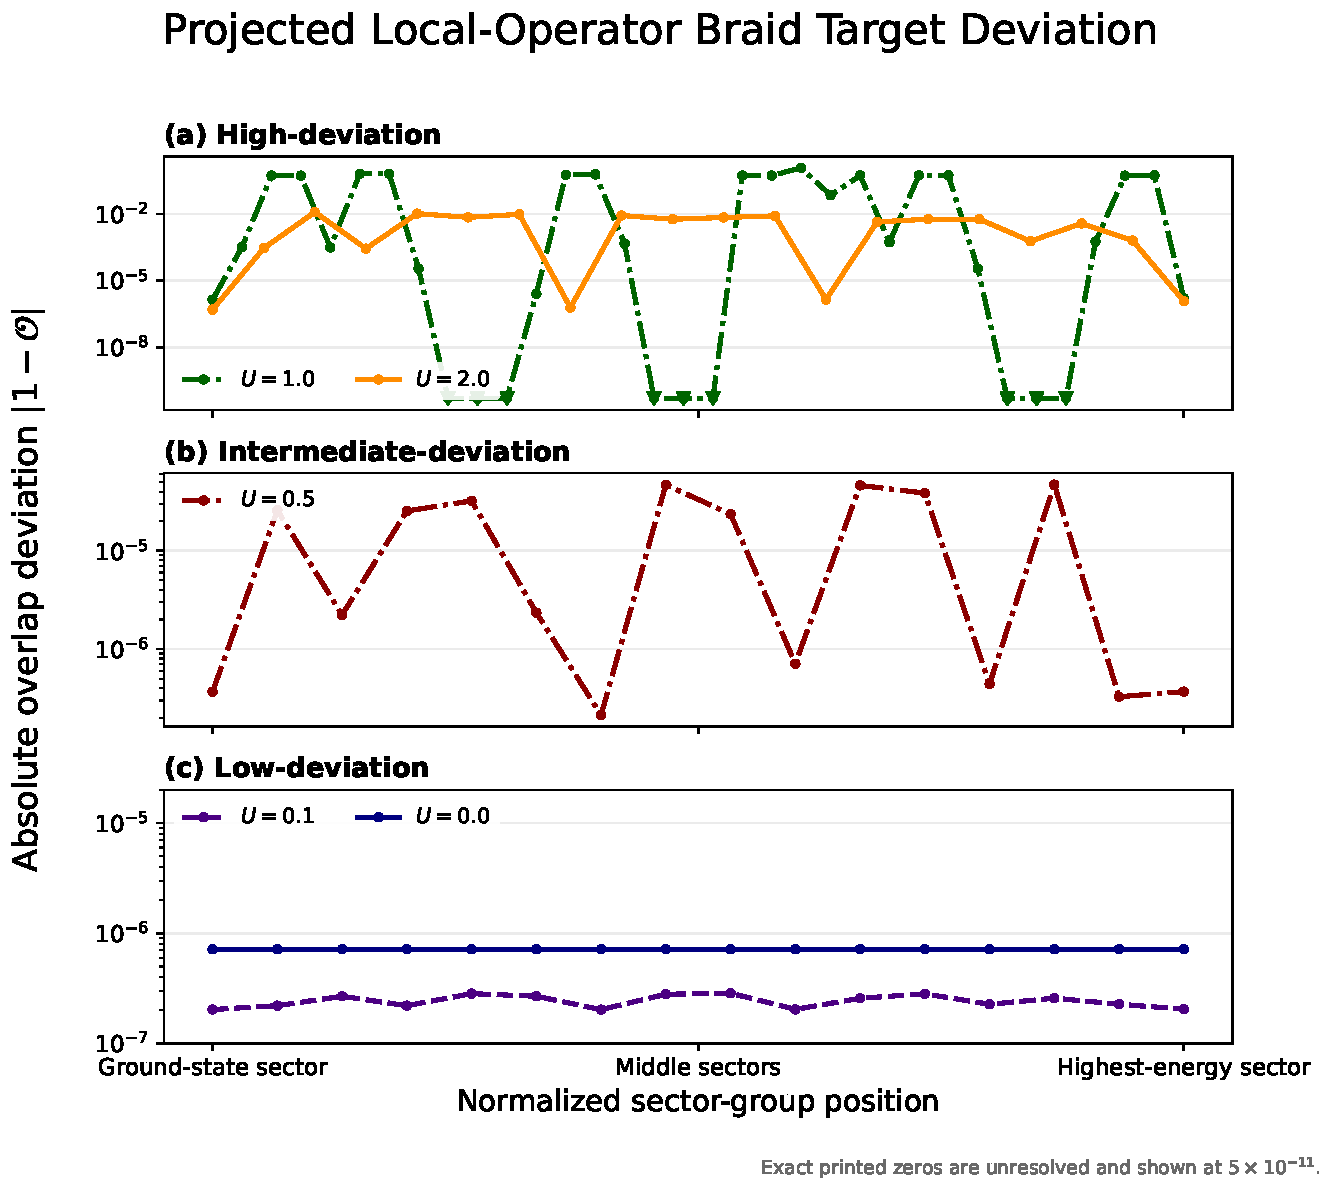
\includegraphics[width=0.9\textwidth]{figs/projected_operator_interaction_regimes.pdf}
  \caption{Self-target braid errors for the projected local-operator model across different energy sectors and interaction strengths $U=0.0$, $U=0.1$, $U=0.5$, $U=1.0$, and $U=2.0$, plotted as the overlap deviation \(D_{\mathcal{O}}=|1-\mathcal{O}|\). The figure is split into three deviation regimes: a) $U=1.0$ and $U=2.0$, b) $U=0.5$, and c) $U=0.0$ and $U=0.1$. The selected weak-interaction configurations have low deviations across all sectors, while the selected stronger-interaction configurations contain sectors with larger self-target errors.}
  \label{fig:projected_operator_interaction_regimes}
\end{figure}
\Cref{fig:projected_operator_interaction_regimes} shows how the self-target braid errors vary among the projected local-operator configurations. The high-deviation panel shows that the selected $U=1.0$ and $U=2.0$ configurations contain sectors with errors as large as order $10^{-1}$ and $10^{-2}$, respectively. Compared with the energy-level Majorana baseline in \cref{fig:ideal_operator_interaction_regimes}, the $U=0.5$ configuration is also more sensitive to sector choice in the projected local-operator model, with errors reaching approximately $10^{-5}$. For $U=0.0$ and $U=0.1$, the errors remain below $10^{-6}$ across all tested sectors. However, because each interaction strength uses a separately optimized parameter set, this trend does not isolate interaction strength as the sole cause.


During the scans, many higher-dimensional energy sectors were found to contain several internal blocks. For example, a $24$-dimensional sector can contain three independent $8\times8$ blocks, as illustrated in \cref{fig:24x24maj}. This matters because a projected local operator does not necessarily have one global orientation across the full sector. In some sectors, the local operator can be fitted to the energy-level Majorana operator with one overall sign across all blocks. In others, different blocks select different relative signs.

To account for this structure, we use the block-matched local-operator model described in \cref{eq:method_block_matched_majorana} and \cref{app:block_label_method}. Each sector scan first fits the projected local operators independently within the labelled blocks. The fitted blocks are then reassembled into one operator on the full sector and used in the braid Hamiltonian.
\begin{figure}[htbp]
  \centering
  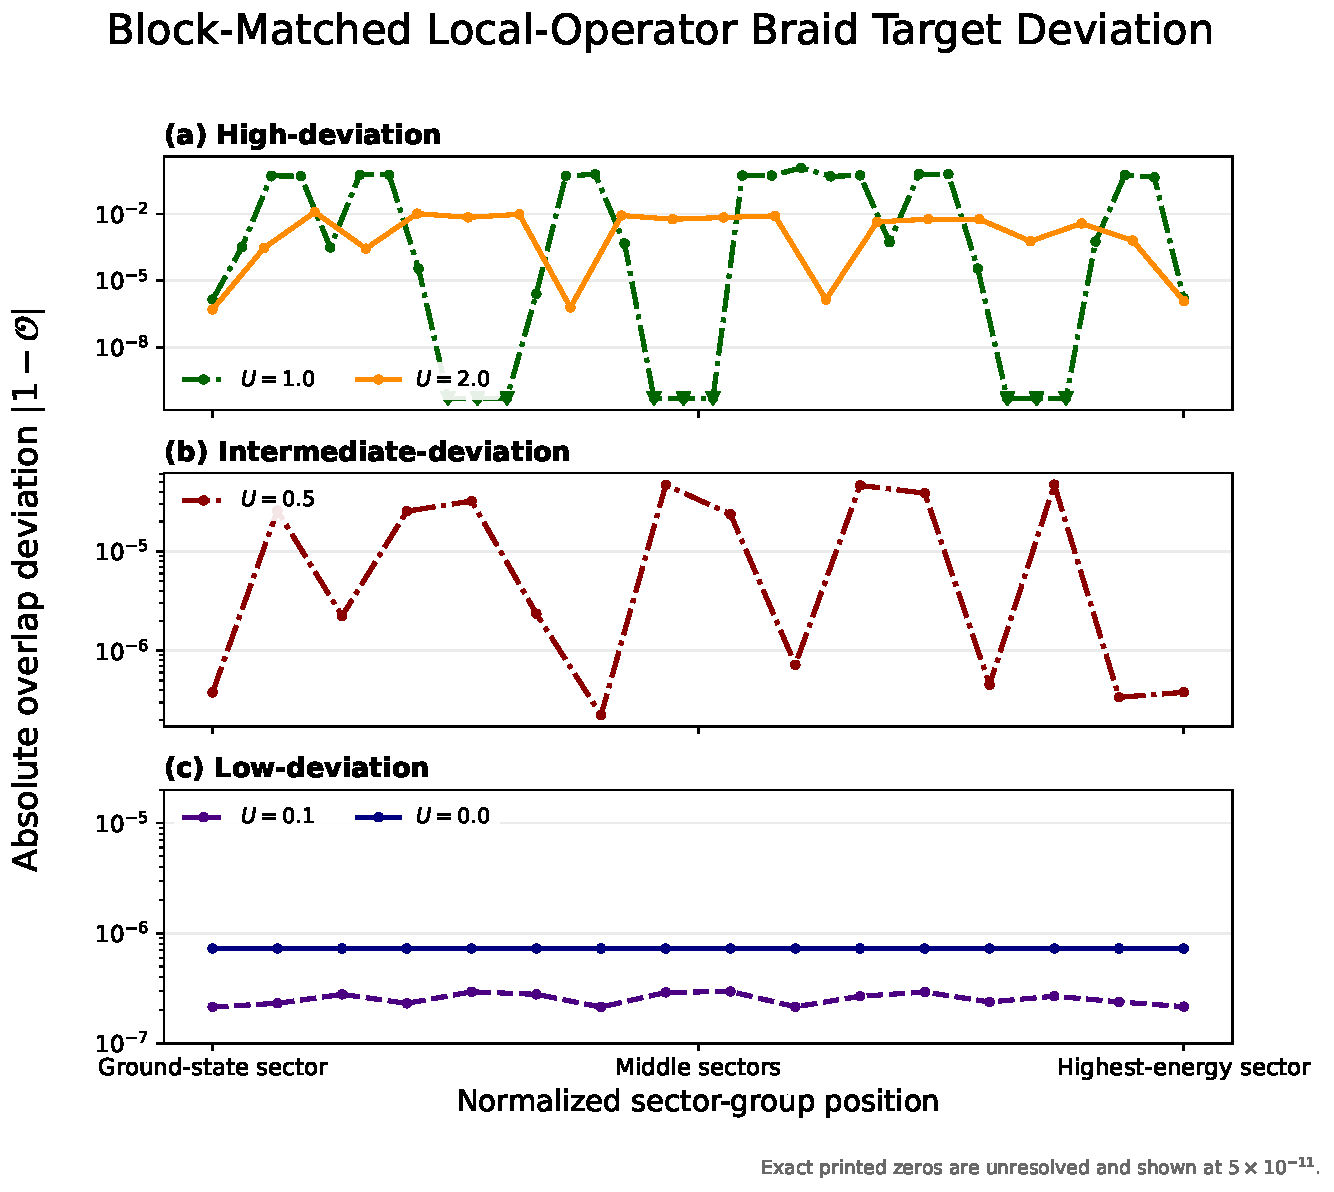
\includegraphics[width=0.9\textwidth]{figs/matched_operator_interaction_regimes.pdf}
  \caption{Self-target braid errors for the block-matched local-operator model, plotted as the overlap deviation \(D_{\mathcal{O}}=|1-\mathcal{O}|\). The same three deviation regimes as in \cref{fig:projected_operator_interaction_regimes} remain visible: a) $U=1.0$ and $U=2.0$, b) $U=0.5$, and c) $U=0.0$ and $U=0.1$.}
  \label{fig:matched_operator_interaction_regimes}
\end{figure}

\Cref{fig:matched_operator_interaction_regimes} shows that the block-matched construction retains the same overall self-target error regimes as the direct projected local-operator model. The $U=0.0$ and $U=0.1$ configurations remain accurate across the tested sectors, while the deviations increase at $U=0.5$ and become larger and more sector dependent for $U=1.0$ and $U=2.0$. Resolving and independently fitting the internal blocks therefore does not by itself remove the sensitivity observed in the local-operator construction.

The resulting blockwise coefficients are reported in \cref{tab:matched_operator_coefficients}. The numerical fitting errors remain between approximately $10^{-15}$ and $10^{-13}$ across all tested interaction strengths, showing that the block-matched operators reproduce the projected local operators essentially exactly. The first-component coefficients are strongly suppressed, so the local endpoint operators remain aligned with the intended second Majorana component rather than rotating into a different energy-level Majorana direction. For $U=0.0$ and $U=0.1$, the fitted second-component coefficients are close to $\pm1$ across all blocks. Small deviations become visible at $U=0.5$, while $U=1.0$ and $U=2.0$ show larger block-dependent variations in magnitude.

The coefficient table also reveals that different blocks within the same sector can select different relative exchange orientations. Since the first-component coefficients vanish at the saved precision, the blockwise braid is controlled mainly by the sign of the product $b_{B,r}b_{C,r}$, as explained in \cref{app:matched_operator_coefficients}. A sector containing both signs does not implement one uniform exchange orientation relative to the energy-level convention. Instead, its fitted target is a direct sum of block-dependent exchange orientations. The individual signs depend on the chosen Majorana sign convention, but their blockwise pattern records how the projected local channels are oriented relative to the fixed energy-level construction.

\begin{figure}[htbp]
  \centering
  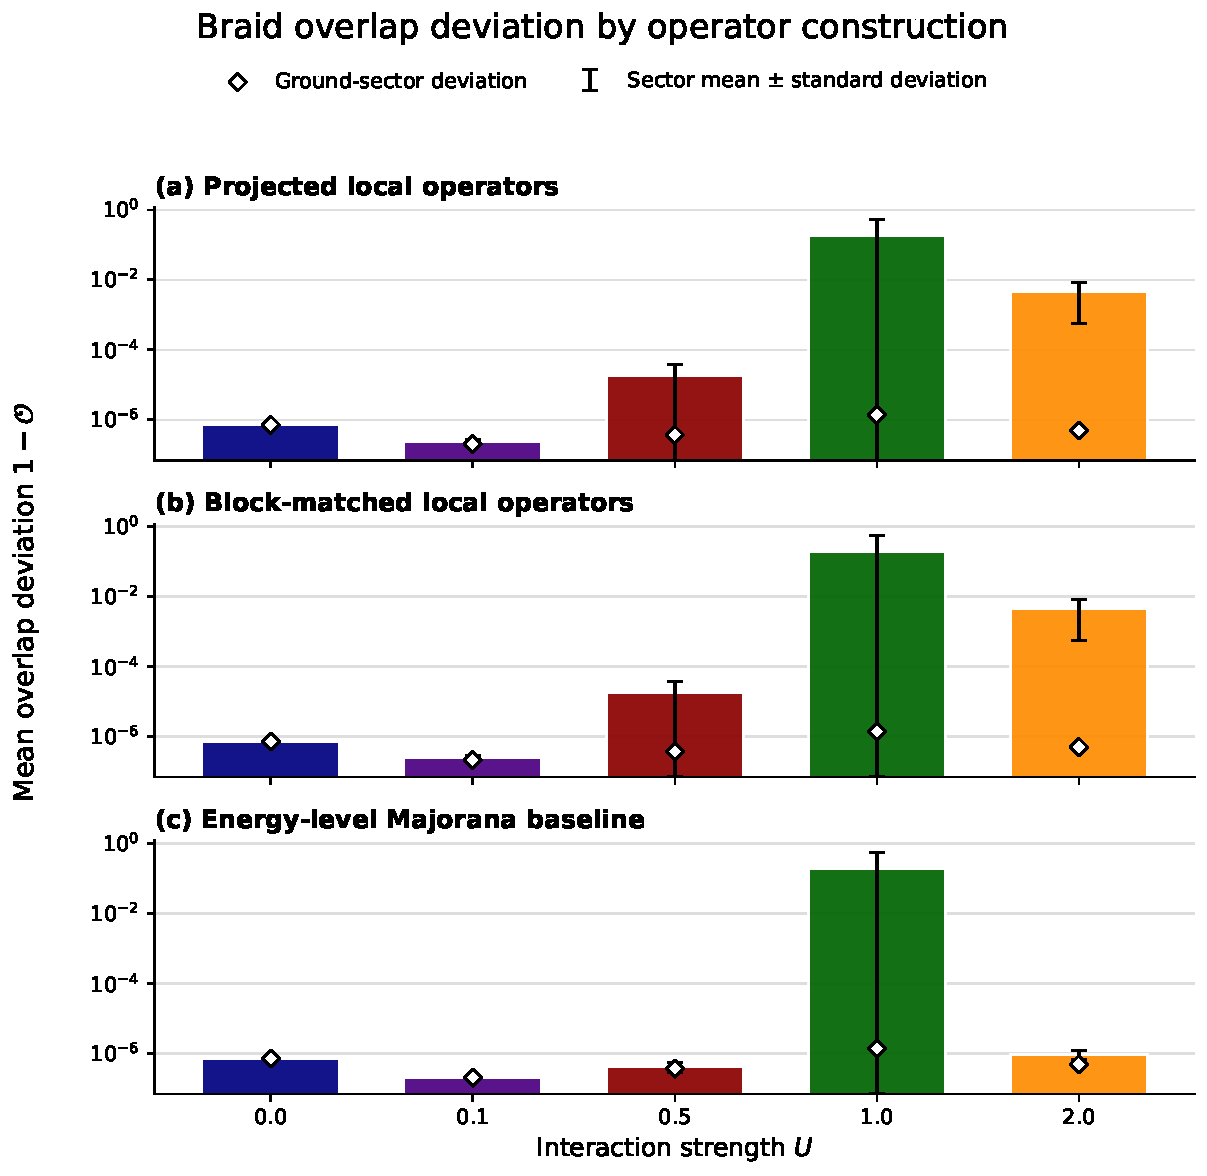
\includegraphics[width=0.9\textwidth]{figs/step_projection_mean_comparison.pdf}
  \caption{Mean self-target braid error across the tested sectors for a) the projected local-operator model, b) the block-matched local-operator model, and c) the energy-level Majorana baseline, using the overlap deviation \(D_{\mathcal{O}}=|1-\mathcal{O}|\). The ground-sector error is marked by a white diamond, and the standard deviation across sectors is shown by a black bar.}
  \label{fig:mean_braid_errors}
\end{figure}
\Cref{fig:mean_braid_errors} summarizes the sector-resolved self-target errors for the projected local-operator model, the block-matched local-operator model, and the energy-level Majorana baseline. For each interaction strength, the bar shows the unweighted mean across the identified sectors, the white diamond marks the ground-sector error, and the black bar shows the sector-to-sector standard deviation. Within these respective target comparisons, the $U=0.1$ and $U=0.0$ configurations have the lowest mean deviations. At $U=0.5$, the local-operator constructions show a noticeable increase in their mean errors, while the energy-level Majorana baseline remains accurate. The worst and most sector-dependent performance occurs at $U=1.0$, while $U=2.0$ is accurate in the energy-level baseline but less accurate in both local-operator constructions.

\newpage
\section{Summary of Main Findings}

The optimization study shows that the PMM chains recover the expected limits while also producing nontrivial interacting configurations. For the non-interacting two-dot system, the optimizer reproduces the known sweet spot, with nearly degenerate parity pairs and edge-localized Majorana polarization. For longer chains, the optimized parameters become increasingly inhomogeneous. In particular, the interior onsite energies are often shifted more strongly than the edge onsite energies. This interior detuning is correlated with favorable edge-localization diagnostics.

The post-optimization diagnostics identify the three-dot system at $U=0.1$ as the strongest interacting braiding candidate. This configuration combines a small ground-state splitting, a large excitation gap, strong opposite-sign edge Majorana polarization, and strongly suppressed bulk polarization. The four-dot system gives a smaller charge difference in the representative weakly interacting case, but it also shows larger ground-state splitting and stronger bulk polarization. Among the tested configurations, the three-dot system therefore provides the best overall compromise between spectral degeneracy and spatial localization. It also decreases the computational cost of the sector-resolved braiding calculations compared with the four-dot system.

The low-energy braiding calculations support this choice. After projection to the lowest manifold, the optimized three-dot building block reproduces the energy-level Majorana operator exchange with high accuracy. The projected microscopic junction operators are dominated by the intended Majorana bilinears, and the energy-level Majorana reference model, the projected microscopic junction model, and the projected local-operator model give nearly identical braid diagnostics in the lowest projected space. This shows that the optimized interacting PMM system can realize the expected Majorana exchange within the controlled low-energy projected model.

Within their respective target comparisons, the sector-resolved scans show low self-target braid errors across all identified energy sectors for the non-interacting and weakly interacting configurations. The energy-level Majorana baseline remains stable for $U=0.0$, $U=0.1$, $U=0.5$, and $U=2.0$, while the selected $U=1.0$ configuration shows large variations between sectors. The direct and block-matched local-operator models are more sensitive in their self-target errors, as these errors increase already at $U=0.5$, and both $U=1.0$ and $U=2.0$ contain less accurate sectors.

The block-matching analysis shows that the projected local operators can be represented essentially exactly within the energy-level Majorana basis. Within each block, the local endpoint operator remains aligned with the intended second Majorana component, while its magnitude and sign can vary between blocks. The relative signs of the two exchanged operators determine whether a block follows the same or opposite exchange orientation relative to the fixed energy-level convention. A sector containing both orientations therefore does not implement one uniform logical exchange across all its internal blocks. Despite resolving this structure, block matching does not substantially change the self-target braid deviations relative to the direct projected local-operator model.

The especially poor and irregular $U=1.0$ result should therefore be treated as a property of the selected optimized configuration, not as evidence that $U=t=1$ is generally worse for braiding than $U=2t$.

For configurations that support a stable exchange channel, the self-target braid accuracy is relatively insensitive to the chosen energy sector. However, the strongly sector-dependent $U=1.0$ result shows that this behavior is not guaranteed and depends on the selected optimized configuration. The differing sector dependence of the energy-level and local constructions leaves a common-target comparison as an important next check before drawing conclusions about how accurately a projected local channel accesses the energy-level exchange.
